% Created by tikzDevice version 0.11 on 2018-07-30 00:20:26
% !TEX encoding = UTF-8 Unicode
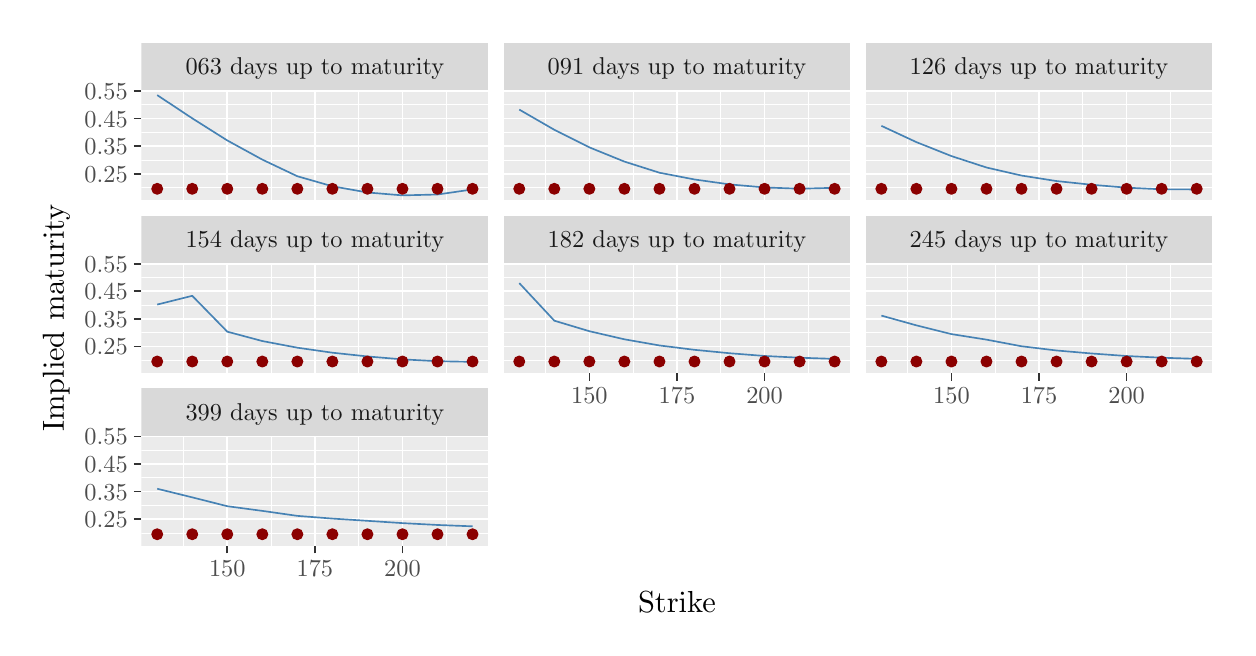
\begin{tikzpicture}[x=1pt,y=1pt]
\definecolor{fillColor}{RGB}{255,255,255}
\path[use as bounding box,fill=fillColor,fill opacity=0.00] (0,0) rectangle (433.62,216.81);
\begin{scope}
\path[clip] (  0.00,  0.00) rectangle (433.62,216.81);
\definecolor{drawColor}{RGB}{255,255,255}
\definecolor{fillColor}{RGB}{255,255,255}

\path[draw=drawColor,line width= 0.6pt,line join=round,line cap=round,fill=fillColor] (  0.00,  0.00) rectangle (433.62,216.81);
\end{scope}
\begin{scope}
\path[clip] ( 41.11,154.40) rectangle (166.45,194.25);
\definecolor{fillColor}{gray}{0.92}

\path[fill=fillColor] ( 41.11,154.40) rectangle (166.45,194.25);
\definecolor{drawColor}{RGB}{255,255,255}

\path[draw=drawColor,line width= 0.3pt,line join=round] ( 41.11,158.99) --
	(166.45,158.99);

\path[draw=drawColor,line width= 0.3pt,line join=round] ( 41.11,168.97) --
	(166.45,168.97);

\path[draw=drawColor,line width= 0.3pt,line join=round] ( 41.11,178.95) --
	(166.45,178.95);

\path[draw=drawColor,line width= 0.3pt,line join=round] ( 41.11,188.93) --
	(166.45,188.93);

\path[draw=drawColor,line width= 0.3pt,line join=round] ( 56.30,154.40) --
	( 56.30,194.25);

\path[draw=drawColor,line width= 0.3pt,line join=round] ( 87.95,154.40) --
	( 87.95,194.25);

\path[draw=drawColor,line width= 0.3pt,line join=round] (119.60,154.40) --
	(119.60,194.25);

\path[draw=drawColor,line width= 0.3pt,line join=round] (151.25,154.40) --
	(151.25,194.25);

\path[draw=drawColor,line width= 0.6pt,line join=round] ( 41.11,163.98) --
	(166.45,163.98);

\path[draw=drawColor,line width= 0.6pt,line join=round] ( 41.11,173.96) --
	(166.45,173.96);

\path[draw=drawColor,line width= 0.6pt,line join=round] ( 41.11,183.94) --
	(166.45,183.94);

\path[draw=drawColor,line width= 0.6pt,line join=round] ( 41.11,193.92) --
	(166.45,193.92);

\path[draw=drawColor,line width= 0.6pt,line join=round] ( 72.13,154.40) --
	( 72.13,194.25);

\path[draw=drawColor,line width= 0.6pt,line join=round] (103.78,154.40) --
	(103.78,194.25);

\path[draw=drawColor,line width= 0.6pt,line join=round] (135.43,154.40) --
	(135.43,194.25);
\definecolor{drawColor}{RGB}{70,130,180}

\path[draw=drawColor,line width= 0.6pt,line join=round] ( 46.81,192.44) --
	( 59.47,184.05) --
	( 72.13,176.06) --
	( 84.79,169.13) --
	( 97.45,163.12) --
	(110.11,159.50) --
	(122.77,157.26) --
	(135.43,156.21) --
	(148.09,156.52) --
	(160.75,158.35);
\definecolor{drawColor}{RGB}{139,0,0}
\definecolor{fillColor}{RGB}{139,0,0}

\path[draw=drawColor,line width= 0.4pt,line join=round,line cap=round,fill=fillColor] ( 46.81,158.58) circle (  1.96);

\path[draw=drawColor,line width= 0.4pt,line join=round,line cap=round,fill=fillColor] ( 59.47,158.58) circle (  1.96);

\path[draw=drawColor,line width= 0.4pt,line join=round,line cap=round,fill=fillColor] ( 72.13,158.58) circle (  1.96);

\path[draw=drawColor,line width= 0.4pt,line join=round,line cap=round,fill=fillColor] ( 84.79,158.58) circle (  1.96);

\path[draw=drawColor,line width= 0.4pt,line join=round,line cap=round,fill=fillColor] ( 97.45,158.58) circle (  1.96);

\path[draw=drawColor,line width= 0.4pt,line join=round,line cap=round,fill=fillColor] (110.11,158.58) circle (  1.96);

\path[draw=drawColor,line width= 0.4pt,line join=round,line cap=round,fill=fillColor] (122.77,158.58) circle (  1.96);

\path[draw=drawColor,line width= 0.4pt,line join=round,line cap=round,fill=fillColor] (135.43,158.58) circle (  1.96);

\path[draw=drawColor,line width= 0.4pt,line join=round,line cap=round,fill=fillColor] (148.09,158.58) circle (  1.96);

\path[draw=drawColor,line width= 0.4pt,line join=round,line cap=round,fill=fillColor] (160.75,158.58) circle (  1.96);
\end{scope}
\begin{scope}
\path[clip] ( 41.11, 91.99) rectangle (166.45,131.84);
\definecolor{fillColor}{gray}{0.92}

\path[fill=fillColor] ( 41.11, 91.99) rectangle (166.45,131.84);
\definecolor{drawColor}{RGB}{255,255,255}

\path[draw=drawColor,line width= 0.3pt,line join=round] ( 41.11, 96.59) --
	(166.45, 96.59);

\path[draw=drawColor,line width= 0.3pt,line join=round] ( 41.11,106.57) --
	(166.45,106.57);

\path[draw=drawColor,line width= 0.3pt,line join=round] ( 41.11,116.55) --
	(166.45,116.55);

\path[draw=drawColor,line width= 0.3pt,line join=round] ( 41.11,126.52) --
	(166.45,126.52);

\path[draw=drawColor,line width= 0.3pt,line join=round] ( 56.30, 91.99) --
	( 56.30,131.84);

\path[draw=drawColor,line width= 0.3pt,line join=round] ( 87.95, 91.99) --
	( 87.95,131.84);

\path[draw=drawColor,line width= 0.3pt,line join=round] (119.60, 91.99) --
	(119.60,131.84);

\path[draw=drawColor,line width= 0.3pt,line join=round] (151.25, 91.99) --
	(151.25,131.84);

\path[draw=drawColor,line width= 0.6pt,line join=round] ( 41.11,101.58) --
	(166.45,101.58);

\path[draw=drawColor,line width= 0.6pt,line join=round] ( 41.11,111.56) --
	(166.45,111.56);

\path[draw=drawColor,line width= 0.6pt,line join=round] ( 41.11,121.54) --
	(166.45,121.54);

\path[draw=drawColor,line width= 0.6pt,line join=round] ( 41.11,131.51) --
	(166.45,131.51);

\path[draw=drawColor,line width= 0.6pt,line join=round] ( 72.13, 91.99) --
	( 72.13,131.84);

\path[draw=drawColor,line width= 0.6pt,line join=round] (103.78, 91.99) --
	(103.78,131.84);

\path[draw=drawColor,line width= 0.6pt,line join=round] (135.43, 91.99) --
	(135.43,131.84);
\definecolor{drawColor}{RGB}{70,130,180}

\path[draw=drawColor,line width= 0.6pt,line join=round] ( 46.81,116.76) --
	( 59.47,119.91) --
	( 72.13,106.96) --
	( 84.79,103.57) --
	( 97.45,101.17) --
	(110.11, 99.36) --
	(122.77, 98.01) --
	(135.43, 96.95) --
	(148.09, 96.29) --
	(160.75, 96.06);
\definecolor{drawColor}{RGB}{139,0,0}
\definecolor{fillColor}{RGB}{139,0,0}

\path[draw=drawColor,line width= 0.4pt,line join=round,line cap=round,fill=fillColor] ( 46.81, 96.17) circle (  1.96);

\path[draw=drawColor,line width= 0.4pt,line join=round,line cap=round,fill=fillColor] ( 59.47, 96.17) circle (  1.96);

\path[draw=drawColor,line width= 0.4pt,line join=round,line cap=round,fill=fillColor] ( 72.13, 96.17) circle (  1.96);

\path[draw=drawColor,line width= 0.4pt,line join=round,line cap=round,fill=fillColor] ( 84.79, 96.17) circle (  1.96);

\path[draw=drawColor,line width= 0.4pt,line join=round,line cap=round,fill=fillColor] ( 97.45, 96.17) circle (  1.96);

\path[draw=drawColor,line width= 0.4pt,line join=round,line cap=round,fill=fillColor] (110.11, 96.17) circle (  1.96);

\path[draw=drawColor,line width= 0.4pt,line join=round,line cap=round,fill=fillColor] (122.77, 96.17) circle (  1.96);

\path[draw=drawColor,line width= 0.4pt,line join=round,line cap=round,fill=fillColor] (135.43, 96.17) circle (  1.96);

\path[draw=drawColor,line width= 0.4pt,line join=round,line cap=round,fill=fillColor] (148.09, 96.17) circle (  1.96);

\path[draw=drawColor,line width= 0.4pt,line join=round,line cap=round,fill=fillColor] (160.75, 96.17) circle (  1.96);
\end{scope}
\begin{scope}
\path[clip] ( 41.11, 29.59) rectangle (166.45, 69.43);
\definecolor{fillColor}{gray}{0.92}

\path[fill=fillColor] ( 41.11, 29.59) rectangle (166.45, 69.43);
\definecolor{drawColor}{RGB}{255,255,255}

\path[draw=drawColor,line width= 0.3pt,line join=round] ( 41.11, 34.18) --
	(166.45, 34.18);

\path[draw=drawColor,line width= 0.3pt,line join=round] ( 41.11, 44.16) --
	(166.45, 44.16);

\path[draw=drawColor,line width= 0.3pt,line join=round] ( 41.11, 54.14) --
	(166.45, 54.14);

\path[draw=drawColor,line width= 0.3pt,line join=round] ( 41.11, 64.12) --
	(166.45, 64.12);

\path[draw=drawColor,line width= 0.3pt,line join=round] ( 56.30, 29.59) --
	( 56.30, 69.43);

\path[draw=drawColor,line width= 0.3pt,line join=round] ( 87.95, 29.59) --
	( 87.95, 69.43);

\path[draw=drawColor,line width= 0.3pt,line join=round] (119.60, 29.59) --
	(119.60, 69.43);

\path[draw=drawColor,line width= 0.3pt,line join=round] (151.25, 29.59) --
	(151.25, 69.43);

\path[draw=drawColor,line width= 0.6pt,line join=round] ( 41.11, 39.17) --
	(166.45, 39.17);

\path[draw=drawColor,line width= 0.6pt,line join=round] ( 41.11, 49.15) --
	(166.45, 49.15);

\path[draw=drawColor,line width= 0.6pt,line join=round] ( 41.11, 59.13) --
	(166.45, 59.13);

\path[draw=drawColor,line width= 0.6pt,line join=round] ( 41.11, 69.11) --
	(166.45, 69.11);

\path[draw=drawColor,line width= 0.6pt,line join=round] ( 72.13, 29.59) --
	( 72.13, 69.43);

\path[draw=drawColor,line width= 0.6pt,line join=round] (103.78, 29.59) --
	(103.78, 69.43);

\path[draw=drawColor,line width= 0.6pt,line join=round] (135.43, 29.59) --
	(135.43, 69.43);
\definecolor{drawColor}{RGB}{70,130,180}

\path[draw=drawColor,line width= 0.6pt,line join=round] ( 46.81, 50.20) --
	( 59.47, 47.09) --
	( 72.13, 43.89) --
	( 84.79, 42.20) --
	( 97.45, 40.40) --
	(110.11, 39.42) --
	(122.77, 38.61) --
	(135.43, 37.78) --
	(148.09, 37.11) --
	(160.75, 36.62);
\definecolor{drawColor}{RGB}{139,0,0}
\definecolor{fillColor}{RGB}{139,0,0}

\path[draw=drawColor,line width= 0.4pt,line join=round,line cap=round,fill=fillColor] ( 46.81, 33.76) circle (  1.96);

\path[draw=drawColor,line width= 0.4pt,line join=round,line cap=round,fill=fillColor] ( 59.47, 33.76) circle (  1.96);

\path[draw=drawColor,line width= 0.4pt,line join=round,line cap=round,fill=fillColor] ( 72.13, 33.76) circle (  1.96);

\path[draw=drawColor,line width= 0.4pt,line join=round,line cap=round,fill=fillColor] ( 84.79, 33.76) circle (  1.96);

\path[draw=drawColor,line width= 0.4pt,line join=round,line cap=round,fill=fillColor] ( 97.45, 33.76) circle (  1.96);

\path[draw=drawColor,line width= 0.4pt,line join=round,line cap=round,fill=fillColor] (110.11, 33.76) circle (  1.96);

\path[draw=drawColor,line width= 0.4pt,line join=round,line cap=round,fill=fillColor] (122.77, 33.76) circle (  1.96);

\path[draw=drawColor,line width= 0.4pt,line join=round,line cap=round,fill=fillColor] (135.43, 33.76) circle (  1.96);

\path[draw=drawColor,line width= 0.4pt,line join=round,line cap=round,fill=fillColor] (148.09, 33.76) circle (  1.96);

\path[draw=drawColor,line width= 0.4pt,line join=round,line cap=round,fill=fillColor] (160.75, 33.76) circle (  1.96);
\end{scope}
\begin{scope}
\path[clip] (171.95,154.40) rectangle (297.28,194.25);
\definecolor{fillColor}{gray}{0.92}

\path[fill=fillColor] (171.95,154.40) rectangle (297.28,194.25);
\definecolor{drawColor}{RGB}{255,255,255}

\path[draw=drawColor,line width= 0.3pt,line join=round] (171.95,158.99) --
	(297.28,158.99);

\path[draw=drawColor,line width= 0.3pt,line join=round] (171.95,168.97) --
	(297.28,168.97);

\path[draw=drawColor,line width= 0.3pt,line join=round] (171.95,178.95) --
	(297.28,178.95);

\path[draw=drawColor,line width= 0.3pt,line join=round] (171.95,188.93) --
	(297.28,188.93);

\path[draw=drawColor,line width= 0.3pt,line join=round] (187.14,154.40) --
	(187.14,194.25);

\path[draw=drawColor,line width= 0.3pt,line join=round] (218.79,154.40) --
	(218.79,194.25);

\path[draw=drawColor,line width= 0.3pt,line join=round] (250.44,154.40) --
	(250.44,194.25);

\path[draw=drawColor,line width= 0.3pt,line join=round] (282.09,154.40) --
	(282.09,194.25);

\path[draw=drawColor,line width= 0.6pt,line join=round] (171.95,163.98) --
	(297.28,163.98);

\path[draw=drawColor,line width= 0.6pt,line join=round] (171.95,173.96) --
	(297.28,173.96);

\path[draw=drawColor,line width= 0.6pt,line join=round] (171.95,183.94) --
	(297.28,183.94);

\path[draw=drawColor,line width= 0.6pt,line join=round] (171.95,193.92) --
	(297.28,193.92);

\path[draw=drawColor,line width= 0.6pt,line join=round] (202.96,154.40) --
	(202.96,194.25);

\path[draw=drawColor,line width= 0.6pt,line join=round] (234.62,154.40) --
	(234.62,194.25);

\path[draw=drawColor,line width= 0.6pt,line join=round] (266.27,154.40) --
	(266.27,194.25);
\definecolor{drawColor}{RGB}{70,130,180}

\path[draw=drawColor,line width= 0.6pt,line join=round] (177.64,187.21) --
	(190.30,179.91) --
	(202.96,173.56) --
	(215.62,168.42) --
	(228.29,164.40) --
	(240.95,161.96) --
	(253.61,160.18) --
	(266.27,159.07) --
	(278.93,158.62) --
	(291.59,158.94);
\definecolor{drawColor}{RGB}{139,0,0}
\definecolor{fillColor}{RGB}{139,0,0}

\path[draw=drawColor,line width= 0.4pt,line join=round,line cap=round,fill=fillColor] (177.64,158.58) circle (  1.96);

\path[draw=drawColor,line width= 0.4pt,line join=round,line cap=round,fill=fillColor] (190.30,158.58) circle (  1.96);

\path[draw=drawColor,line width= 0.4pt,line join=round,line cap=round,fill=fillColor] (202.96,158.58) circle (  1.96);

\path[draw=drawColor,line width= 0.4pt,line join=round,line cap=round,fill=fillColor] (215.62,158.58) circle (  1.96);

\path[draw=drawColor,line width= 0.4pt,line join=round,line cap=round,fill=fillColor] (228.29,158.58) circle (  1.96);

\path[draw=drawColor,line width= 0.4pt,line join=round,line cap=round,fill=fillColor] (240.95,158.58) circle (  1.96);

\path[draw=drawColor,line width= 0.4pt,line join=round,line cap=round,fill=fillColor] (253.61,158.58) circle (  1.96);

\path[draw=drawColor,line width= 0.4pt,line join=round,line cap=round,fill=fillColor] (266.27,158.58) circle (  1.96);

\path[draw=drawColor,line width= 0.4pt,line join=round,line cap=round,fill=fillColor] (278.93,158.58) circle (  1.96);

\path[draw=drawColor,line width= 0.4pt,line join=round,line cap=round,fill=fillColor] (291.59,158.58) circle (  1.96);
\end{scope}
\begin{scope}
\path[clip] (171.95, 91.99) rectangle (297.28,131.84);
\definecolor{fillColor}{gray}{0.92}

\path[fill=fillColor] (171.95, 91.99) rectangle (297.28,131.84);
\definecolor{drawColor}{RGB}{255,255,255}

\path[draw=drawColor,line width= 0.3pt,line join=round] (171.95, 96.59) --
	(297.28, 96.59);

\path[draw=drawColor,line width= 0.3pt,line join=round] (171.95,106.57) --
	(297.28,106.57);

\path[draw=drawColor,line width= 0.3pt,line join=round] (171.95,116.55) --
	(297.28,116.55);

\path[draw=drawColor,line width= 0.3pt,line join=round] (171.95,126.52) --
	(297.28,126.52);

\path[draw=drawColor,line width= 0.3pt,line join=round] (187.14, 91.99) --
	(187.14,131.84);

\path[draw=drawColor,line width= 0.3pt,line join=round] (218.79, 91.99) --
	(218.79,131.84);

\path[draw=drawColor,line width= 0.3pt,line join=round] (250.44, 91.99) --
	(250.44,131.84);

\path[draw=drawColor,line width= 0.3pt,line join=round] (282.09, 91.99) --
	(282.09,131.84);

\path[draw=drawColor,line width= 0.6pt,line join=round] (171.95,101.58) --
	(297.28,101.58);

\path[draw=drawColor,line width= 0.6pt,line join=round] (171.95,111.56) --
	(297.28,111.56);

\path[draw=drawColor,line width= 0.6pt,line join=round] (171.95,121.54) --
	(297.28,121.54);

\path[draw=drawColor,line width= 0.6pt,line join=round] (171.95,131.51) --
	(297.28,131.51);

\path[draw=drawColor,line width= 0.6pt,line join=round] (202.96, 91.99) --
	(202.96,131.84);

\path[draw=drawColor,line width= 0.6pt,line join=round] (234.62, 91.99) --
	(234.62,131.84);

\path[draw=drawColor,line width= 0.6pt,line join=round] (266.27, 91.99) --
	(266.27,131.84);
\definecolor{drawColor}{RGB}{70,130,180}

\path[draw=drawColor,line width= 0.6pt,line join=round] (177.64,124.51) --
	(190.30,110.93) --
	(202.96,107.13) --
	(215.62,104.20) --
	(228.29,101.98) --
	(240.95,100.40) --
	(253.61, 99.17) --
	(266.27, 98.18) --
	(278.93, 97.55) --
	(291.59, 97.12);
\definecolor{drawColor}{RGB}{139,0,0}
\definecolor{fillColor}{RGB}{139,0,0}

\path[draw=drawColor,line width= 0.4pt,line join=round,line cap=round,fill=fillColor] (177.64, 96.17) circle (  1.96);

\path[draw=drawColor,line width= 0.4pt,line join=round,line cap=round,fill=fillColor] (190.30, 96.17) circle (  1.96);

\path[draw=drawColor,line width= 0.4pt,line join=round,line cap=round,fill=fillColor] (202.96, 96.17) circle (  1.96);

\path[draw=drawColor,line width= 0.4pt,line join=round,line cap=round,fill=fillColor] (215.62, 96.17) circle (  1.96);

\path[draw=drawColor,line width= 0.4pt,line join=round,line cap=round,fill=fillColor] (228.29, 96.17) circle (  1.96);

\path[draw=drawColor,line width= 0.4pt,line join=round,line cap=round,fill=fillColor] (240.95, 96.17) circle (  1.96);

\path[draw=drawColor,line width= 0.4pt,line join=round,line cap=round,fill=fillColor] (253.61, 96.17) circle (  1.96);

\path[draw=drawColor,line width= 0.4pt,line join=round,line cap=round,fill=fillColor] (266.27, 96.17) circle (  1.96);

\path[draw=drawColor,line width= 0.4pt,line join=round,line cap=round,fill=fillColor] (278.93, 96.17) circle (  1.96);

\path[draw=drawColor,line width= 0.4pt,line join=round,line cap=round,fill=fillColor] (291.59, 96.17) circle (  1.96);
\end{scope}
\begin{scope}
\path[clip] (302.78,154.40) rectangle (428.12,194.25);
\definecolor{fillColor}{gray}{0.92}

\path[fill=fillColor] (302.78,154.40) rectangle (428.12,194.25);
\definecolor{drawColor}{RGB}{255,255,255}

\path[draw=drawColor,line width= 0.3pt,line join=round] (302.78,158.99) --
	(428.12,158.99);

\path[draw=drawColor,line width= 0.3pt,line join=round] (302.78,168.97) --
	(428.12,168.97);

\path[draw=drawColor,line width= 0.3pt,line join=round] (302.78,178.95) --
	(428.12,178.95);

\path[draw=drawColor,line width= 0.3pt,line join=round] (302.78,188.93) --
	(428.12,188.93);

\path[draw=drawColor,line width= 0.3pt,line join=round] (317.98,154.40) --
	(317.98,194.25);

\path[draw=drawColor,line width= 0.3pt,line join=round] (349.63,154.40) --
	(349.63,194.25);

\path[draw=drawColor,line width= 0.3pt,line join=round] (381.28,154.40) --
	(381.28,194.25);

\path[draw=drawColor,line width= 0.3pt,line join=round] (412.93,154.40) --
	(412.93,194.25);

\path[draw=drawColor,line width= 0.6pt,line join=round] (302.78,163.98) --
	(428.12,163.98);

\path[draw=drawColor,line width= 0.6pt,line join=round] (302.78,173.96) --
	(428.12,173.96);

\path[draw=drawColor,line width= 0.6pt,line join=round] (302.78,183.94) --
	(428.12,183.94);

\path[draw=drawColor,line width= 0.6pt,line join=round] (302.78,193.92) --
	(428.12,193.92);

\path[draw=drawColor,line width= 0.6pt,line join=round] (333.80,154.40) --
	(333.80,194.25);

\path[draw=drawColor,line width= 0.6pt,line join=round] (365.45,154.40) --
	(365.45,194.25);

\path[draw=drawColor,line width= 0.6pt,line join=round] (397.10,154.40) --
	(397.10,194.25);
\definecolor{drawColor}{RGB}{70,130,180}

\path[draw=drawColor,line width= 0.6pt,line join=round] (308.48,181.34) --
	(321.14,175.45) --
	(333.80,170.41) --
	(346.46,166.28) --
	(359.12,163.37) --
	(371.78,161.38) --
	(384.44,160.05) --
	(397.10,158.99) --
	(409.76,158.40) --
	(422.42,158.35);
\definecolor{drawColor}{RGB}{139,0,0}
\definecolor{fillColor}{RGB}{139,0,0}

\path[draw=drawColor,line width= 0.4pt,line join=round,line cap=round,fill=fillColor] (308.48,158.58) circle (  1.96);

\path[draw=drawColor,line width= 0.4pt,line join=round,line cap=round,fill=fillColor] (321.14,158.58) circle (  1.96);

\path[draw=drawColor,line width= 0.4pt,line join=round,line cap=round,fill=fillColor] (333.80,158.58) circle (  1.96);

\path[draw=drawColor,line width= 0.4pt,line join=round,line cap=round,fill=fillColor] (346.46,158.58) circle (  1.96);

\path[draw=drawColor,line width= 0.4pt,line join=round,line cap=round,fill=fillColor] (359.12,158.58) circle (  1.96);

\path[draw=drawColor,line width= 0.4pt,line join=round,line cap=round,fill=fillColor] (371.78,158.58) circle (  1.96);

\path[draw=drawColor,line width= 0.4pt,line join=round,line cap=round,fill=fillColor] (384.44,158.58) circle (  1.96);

\path[draw=drawColor,line width= 0.4pt,line join=round,line cap=round,fill=fillColor] (397.10,158.58) circle (  1.96);

\path[draw=drawColor,line width= 0.4pt,line join=round,line cap=round,fill=fillColor] (409.76,158.58) circle (  1.96);

\path[draw=drawColor,line width= 0.4pt,line join=round,line cap=round,fill=fillColor] (422.42,158.58) circle (  1.96);
\end{scope}
\begin{scope}
\path[clip] (302.78, 91.99) rectangle (428.12,131.84);
\definecolor{fillColor}{gray}{0.92}

\path[fill=fillColor] (302.78, 91.99) rectangle (428.12,131.84);
\definecolor{drawColor}{RGB}{255,255,255}

\path[draw=drawColor,line width= 0.3pt,line join=round] (302.78, 96.59) --
	(428.12, 96.59);

\path[draw=drawColor,line width= 0.3pt,line join=round] (302.78,106.57) --
	(428.12,106.57);

\path[draw=drawColor,line width= 0.3pt,line join=round] (302.78,116.55) --
	(428.12,116.55);

\path[draw=drawColor,line width= 0.3pt,line join=round] (302.78,126.52) --
	(428.12,126.52);

\path[draw=drawColor,line width= 0.3pt,line join=round] (317.98, 91.99) --
	(317.98,131.84);

\path[draw=drawColor,line width= 0.3pt,line join=round] (349.63, 91.99) --
	(349.63,131.84);

\path[draw=drawColor,line width= 0.3pt,line join=round] (381.28, 91.99) --
	(381.28,131.84);

\path[draw=drawColor,line width= 0.3pt,line join=round] (412.93, 91.99) --
	(412.93,131.84);

\path[draw=drawColor,line width= 0.6pt,line join=round] (302.78,101.58) --
	(428.12,101.58);

\path[draw=drawColor,line width= 0.6pt,line join=round] (302.78,111.56) --
	(428.12,111.56);

\path[draw=drawColor,line width= 0.6pt,line join=round] (302.78,121.54) --
	(428.12,121.54);

\path[draw=drawColor,line width= 0.6pt,line join=round] (302.78,131.51) --
	(428.12,131.51);

\path[draw=drawColor,line width= 0.6pt,line join=round] (333.80, 91.99) --
	(333.80,131.84);

\path[draw=drawColor,line width= 0.6pt,line join=round] (365.45, 91.99) --
	(365.45,131.84);

\path[draw=drawColor,line width= 0.6pt,line join=round] (397.10, 91.99) --
	(397.10,131.84);
\definecolor{drawColor}{RGB}{70,130,180}

\path[draw=drawColor,line width= 0.6pt,line join=round] (308.48,112.77) --
	(321.14,109.24) --
	(333.80,106.08) --
	(346.46,104.08) --
	(359.12,101.69) --
	(371.78,100.16) --
	(384.44, 99.08) --
	(397.10, 98.16) --
	(409.76, 97.55) --
	(422.42, 97.14);
\definecolor{drawColor}{RGB}{139,0,0}
\definecolor{fillColor}{RGB}{139,0,0}

\path[draw=drawColor,line width= 0.4pt,line join=round,line cap=round,fill=fillColor] (308.48, 96.17) circle (  1.96);

\path[draw=drawColor,line width= 0.4pt,line join=round,line cap=round,fill=fillColor] (321.14, 96.17) circle (  1.96);

\path[draw=drawColor,line width= 0.4pt,line join=round,line cap=round,fill=fillColor] (333.80, 96.17) circle (  1.96);

\path[draw=drawColor,line width= 0.4pt,line join=round,line cap=round,fill=fillColor] (346.46, 96.17) circle (  1.96);

\path[draw=drawColor,line width= 0.4pt,line join=round,line cap=round,fill=fillColor] (359.12, 96.17) circle (  1.96);

\path[draw=drawColor,line width= 0.4pt,line join=round,line cap=round,fill=fillColor] (371.78, 96.17) circle (  1.96);

\path[draw=drawColor,line width= 0.4pt,line join=round,line cap=round,fill=fillColor] (384.44, 96.17) circle (  1.96);

\path[draw=drawColor,line width= 0.4pt,line join=round,line cap=round,fill=fillColor] (397.10, 96.17) circle (  1.96);

\path[draw=drawColor,line width= 0.4pt,line join=round,line cap=round,fill=fillColor] (409.76, 96.17) circle (  1.96);

\path[draw=drawColor,line width= 0.4pt,line join=round,line cap=round,fill=fillColor] (422.42, 96.17) circle (  1.96);
\end{scope}
\begin{scope}
\path[clip] ( 41.11, 69.43) rectangle (166.45, 86.49);
\definecolor{fillColor}{gray}{0.85}

\path[fill=fillColor] ( 41.11, 69.43) rectangle (166.45, 86.49);
\definecolor{drawColor}{gray}{0.10}

\node[text=drawColor,anchor=base,inner sep=0pt, outer sep=0pt, scale=  0.88] at (103.78, 74.93) {399 days up to maturity};
\end{scope}
\begin{scope}
\path[clip] ( 41.11,131.84) rectangle (166.45,148.90);
\definecolor{fillColor}{gray}{0.85}

\path[fill=fillColor] ( 41.11,131.84) rectangle (166.45,148.90);
\definecolor{drawColor}{gray}{0.10}

\node[text=drawColor,anchor=base,inner sep=0pt, outer sep=0pt, scale=  0.88] at (103.78,137.34) {154 days up to maturity};
\end{scope}
\begin{scope}
\path[clip] (171.95,131.84) rectangle (297.28,148.90);
\definecolor{fillColor}{gray}{0.85}

\path[fill=fillColor] (171.95,131.84) rectangle (297.28,148.90);
\definecolor{drawColor}{gray}{0.10}

\node[text=drawColor,anchor=base,inner sep=0pt, outer sep=0pt, scale=  0.88] at (234.62,137.34) {182 days up to maturity};
\end{scope}
\begin{scope}
\path[clip] (302.78,131.84) rectangle (428.12,148.90);
\definecolor{fillColor}{gray}{0.85}

\path[fill=fillColor] (302.78,131.84) rectangle (428.12,148.90);
\definecolor{drawColor}{gray}{0.10}

\node[text=drawColor,anchor=base,inner sep=0pt, outer sep=0pt, scale=  0.88] at (365.45,137.34) {245 days up to maturity};
\end{scope}
\begin{scope}
\path[clip] ( 41.11,194.25) rectangle (166.45,211.31);
\definecolor{fillColor}{gray}{0.85}

\path[fill=fillColor] ( 41.11,194.25) rectangle (166.45,211.31);
\definecolor{drawColor}{gray}{0.10}

\node[text=drawColor,anchor=base,inner sep=0pt, outer sep=0pt, scale=  0.88] at (103.78,199.75) {063 days up to maturity};
\end{scope}
\begin{scope}
\path[clip] (171.95,194.25) rectangle (297.28,211.31);
\definecolor{fillColor}{gray}{0.85}

\path[fill=fillColor] (171.95,194.25) rectangle (297.28,211.31);
\definecolor{drawColor}{gray}{0.10}

\node[text=drawColor,anchor=base,inner sep=0pt, outer sep=0pt, scale=  0.88] at (234.62,199.75) {091 days up to maturity};
\end{scope}
\begin{scope}
\path[clip] (302.78,194.25) rectangle (428.12,211.31);
\definecolor{fillColor}{gray}{0.85}

\path[fill=fillColor] (302.78,194.25) rectangle (428.12,211.31);
\definecolor{drawColor}{gray}{0.10}

\node[text=drawColor,anchor=base,inner sep=0pt, outer sep=0pt, scale=  0.88] at (365.45,199.75) {126 days up to maturity};
\end{scope}
\begin{scope}
\path[clip] (  0.00,  0.00) rectangle (433.62,216.81);
\definecolor{drawColor}{gray}{0.20}

\path[draw=drawColor,line width= 0.6pt,line join=round] ( 72.13, 26.84) --
	( 72.13, 29.59);

\path[draw=drawColor,line width= 0.6pt,line join=round] (103.78, 26.84) --
	(103.78, 29.59);

\path[draw=drawColor,line width= 0.6pt,line join=round] (135.43, 26.84) --
	(135.43, 29.59);
\end{scope}
\begin{scope}
\path[clip] (  0.00,  0.00) rectangle (433.62,216.81);
\definecolor{drawColor}{gray}{0.30}

\node[text=drawColor,anchor=base,inner sep=0pt, outer sep=0pt, scale=  0.88] at ( 72.13, 18.58) {150};

\node[text=drawColor,anchor=base,inner sep=0pt, outer sep=0pt, scale=  0.88] at (103.78, 18.58) {175};

\node[text=drawColor,anchor=base,inner sep=0pt, outer sep=0pt, scale=  0.88] at (135.43, 18.58) {200};
\end{scope}
\begin{scope}
\path[clip] (  0.00,  0.00) rectangle (433.62,216.81);
\definecolor{drawColor}{gray}{0.20}

\path[draw=drawColor,line width= 0.6pt,line join=round] (202.96, 89.24) --
	(202.96, 91.99);

\path[draw=drawColor,line width= 0.6pt,line join=round] (234.62, 89.24) --
	(234.62, 91.99);

\path[draw=drawColor,line width= 0.6pt,line join=round] (266.27, 89.24) --
	(266.27, 91.99);
\end{scope}
\begin{scope}
\path[clip] (  0.00,  0.00) rectangle (433.62,216.81);
\definecolor{drawColor}{gray}{0.30}

\node[text=drawColor,anchor=base,inner sep=0pt, outer sep=0pt, scale=  0.88] at (202.96, 80.98) {150};

\node[text=drawColor,anchor=base,inner sep=0pt, outer sep=0pt, scale=  0.88] at (234.62, 80.98) {175};

\node[text=drawColor,anchor=base,inner sep=0pt, outer sep=0pt, scale=  0.88] at (266.27, 80.98) {200};
\end{scope}
\begin{scope}
\path[clip] (  0.00,  0.00) rectangle (433.62,216.81);
\definecolor{drawColor}{gray}{0.20}

\path[draw=drawColor,line width= 0.6pt,line join=round] (333.80, 89.24) --
	(333.80, 91.99);

\path[draw=drawColor,line width= 0.6pt,line join=round] (365.45, 89.24) --
	(365.45, 91.99);

\path[draw=drawColor,line width= 0.6pt,line join=round] (397.10, 89.24) --
	(397.10, 91.99);
\end{scope}
\begin{scope}
\path[clip] (  0.00,  0.00) rectangle (433.62,216.81);
\definecolor{drawColor}{gray}{0.30}

\node[text=drawColor,anchor=base,inner sep=0pt, outer sep=0pt, scale=  0.88] at (333.80, 80.98) {150};

\node[text=drawColor,anchor=base,inner sep=0pt, outer sep=0pt, scale=  0.88] at (365.45, 80.98) {175};

\node[text=drawColor,anchor=base,inner sep=0pt, outer sep=0pt, scale=  0.88] at (397.10, 80.98) {200};
\end{scope}
\begin{scope}
\path[clip] (  0.00,  0.00) rectangle (433.62,216.81);
\definecolor{drawColor}{gray}{0.30}

\node[text=drawColor,anchor=base east,inner sep=0pt, outer sep=0pt, scale=  0.88] at ( 36.16,160.95) {0.25};

\node[text=drawColor,anchor=base east,inner sep=0pt, outer sep=0pt, scale=  0.88] at ( 36.16,170.93) {0.35};

\node[text=drawColor,anchor=base east,inner sep=0pt, outer sep=0pt, scale=  0.88] at ( 36.16,180.91) {0.45};

\node[text=drawColor,anchor=base east,inner sep=0pt, outer sep=0pt, scale=  0.88] at ( 36.16,190.89) {0.55};
\end{scope}
\begin{scope}
\path[clip] (  0.00,  0.00) rectangle (433.62,216.81);
\definecolor{drawColor}{gray}{0.20}

\path[draw=drawColor,line width= 0.6pt,line join=round] ( 38.36,163.98) --
	( 41.11,163.98);

\path[draw=drawColor,line width= 0.6pt,line join=round] ( 38.36,173.96) --
	( 41.11,173.96);

\path[draw=drawColor,line width= 0.6pt,line join=round] ( 38.36,183.94) --
	( 41.11,183.94);

\path[draw=drawColor,line width= 0.6pt,line join=round] ( 38.36,193.92) --
	( 41.11,193.92);
\end{scope}
\begin{scope}
\path[clip] (  0.00,  0.00) rectangle (433.62,216.81);
\definecolor{drawColor}{gray}{0.30}

\node[text=drawColor,anchor=base east,inner sep=0pt, outer sep=0pt, scale=  0.88] at ( 36.16, 98.55) {0.25};

\node[text=drawColor,anchor=base east,inner sep=0pt, outer sep=0pt, scale=  0.88] at ( 36.16,108.52) {0.35};

\node[text=drawColor,anchor=base east,inner sep=0pt, outer sep=0pt, scale=  0.88] at ( 36.16,118.50) {0.45};

\node[text=drawColor,anchor=base east,inner sep=0pt, outer sep=0pt, scale=  0.88] at ( 36.16,128.48) {0.55};
\end{scope}
\begin{scope}
\path[clip] (  0.00,  0.00) rectangle (433.62,216.81);
\definecolor{drawColor}{gray}{0.20}

\path[draw=drawColor,line width= 0.6pt,line join=round] ( 38.36,101.58) --
	( 41.11,101.58);

\path[draw=drawColor,line width= 0.6pt,line join=round] ( 38.36,111.56) --
	( 41.11,111.56);

\path[draw=drawColor,line width= 0.6pt,line join=round] ( 38.36,121.54) --
	( 41.11,121.54);

\path[draw=drawColor,line width= 0.6pt,line join=round] ( 38.36,131.51) --
	( 41.11,131.51);
\end{scope}
\begin{scope}
\path[clip] (  0.00,  0.00) rectangle (433.62,216.81);
\definecolor{drawColor}{gray}{0.30}

\node[text=drawColor,anchor=base east,inner sep=0pt, outer sep=0pt, scale=  0.88] at ( 36.16, 36.14) {0.25};

\node[text=drawColor,anchor=base east,inner sep=0pt, outer sep=0pt, scale=  0.88] at ( 36.16, 46.12) {0.35};

\node[text=drawColor,anchor=base east,inner sep=0pt, outer sep=0pt, scale=  0.88] at ( 36.16, 56.10) {0.45};

\node[text=drawColor,anchor=base east,inner sep=0pt, outer sep=0pt, scale=  0.88] at ( 36.16, 66.08) {0.55};
\end{scope}
\begin{scope}
\path[clip] (  0.00,  0.00) rectangle (433.62,216.81);
\definecolor{drawColor}{gray}{0.20}

\path[draw=drawColor,line width= 0.6pt,line join=round] ( 38.36, 39.17) --
	( 41.11, 39.17);

\path[draw=drawColor,line width= 0.6pt,line join=round] ( 38.36, 49.15) --
	( 41.11, 49.15);

\path[draw=drawColor,line width= 0.6pt,line join=round] ( 38.36, 59.13) --
	( 41.11, 59.13);

\path[draw=drawColor,line width= 0.6pt,line join=round] ( 38.36, 69.11) --
	( 41.11, 69.11);
\end{scope}
\begin{scope}
\path[clip] (  0.00,  0.00) rectangle (433.62,216.81);
\definecolor{drawColor}{RGB}{0,0,0}

\node[text=drawColor,anchor=base,inner sep=0pt, outer sep=0pt, scale=  1.10] at (234.62,  5.50) {Strike};
\end{scope}
\begin{scope}
\path[clip] (  0.00,  0.00) rectangle (433.62,216.81);
\definecolor{drawColor}{RGB}{0,0,0}

\node[text=drawColor,rotate= 90.00,anchor=base,inner sep=0pt, outer sep=0pt, scale=  1.10] at ( 13.08,111.92) {Implied maturity};
\end{scope}
\end{tikzpicture}
